\chapter{Design}

Il presente capitolo descrive le scelte architetturali, tecnologiche e progettuali adottate per soddisfare gli obiettivi e i requisiti definiti nel capitolo precedente. L'attenzione si concentra sulle funzionalità sviluppate o analizzate durante il tirocinio, pur accennando alle linee guida per alcune delle funzionalità future, al fine di offrire una visione più completa del sistema.

La progettazione del nuovo sistema punta a superare i limiti identificati nel legacy, adottando un'architettura moderna, modulare e scalabile, che semplifichi la gestione e consenta l'integrazione di nuove funzionalità. Particolare attenzione è stata dedicata alla separazione delle responsabilità tra i vari componenti, alla progettazione di un backend flessibile e robusto agli errori, e alla realizzazione di un frontend intuitivo e con un aspetto enterprise.

Il capitolo è strutturato come segue: dopo una descrizione dell’architettura generale del sistema, si approfondiranno le principali componenti e funzionalità chiave, come la multiutenza e la gestione degli errori. Infine, saranno discussi gli aspetti relativi al miglioramento del database e alle strategie messe in campo per garantire una corretta migrazione dei dati dal sistema legacy.

\section{Architettura generale} Per la progettazione del nuovo sistema è stata adottata un'architettura a microservizi, caratterizzata da una separazione netta tra frontend e backend. Questa scelta è motivata dalla necessità di superare i limiti architetturali del sistema legacy, introducendo modularità e una chiara separazione delle responsabilità tra i vari componenti.

Nel nuovo sistema, il frontend è rappresentato da un singolo microservizio dedicato alla logica di presentazione dei dati e all'interazione con l'utente. Il backend, invece, è stato suddiviso in molteplici microservizi indipendenti, ciascuno dedicato a un modulo o a una funzionalità specifica dell'applicativo. Questa scomposizione consente di ottenere una maggiore flessibilità, facilitando sia l'aggiunta di nuove funzionalità che la manutenzione del sistema.

I microservizi comunicano tra loro utilizzando il protocollo HTTP e, più specificamente, attraverso le API RESTful che ciascuno di essi espone. Queste ultime vengono inoltre utilizzate sia dal frontend sia per la creazione delle API pubbliche aziendali. Tali API, già presenti insieme al sistema legacy, sono state rinnovate per adattarsi alle nuove logiche di funzionamento introdotte nel nuovo sistema.

Una rappresentazione schematica dell'architettura del sistema è riportata in \Cref{fig:system-architecture}, dove sono evidenziate le principali componenti del frontend e del backend. Il diagramma mostra come il primo gestisca l'interazione con l'utente attraverso moduli specifici per il routing e per la gestione dello stato e della sessione, mentre il secondo sia organizzato in servizi dedicati a funzionalità come gestione utenti e autenticazione.

\begin{figure}
  \centering
  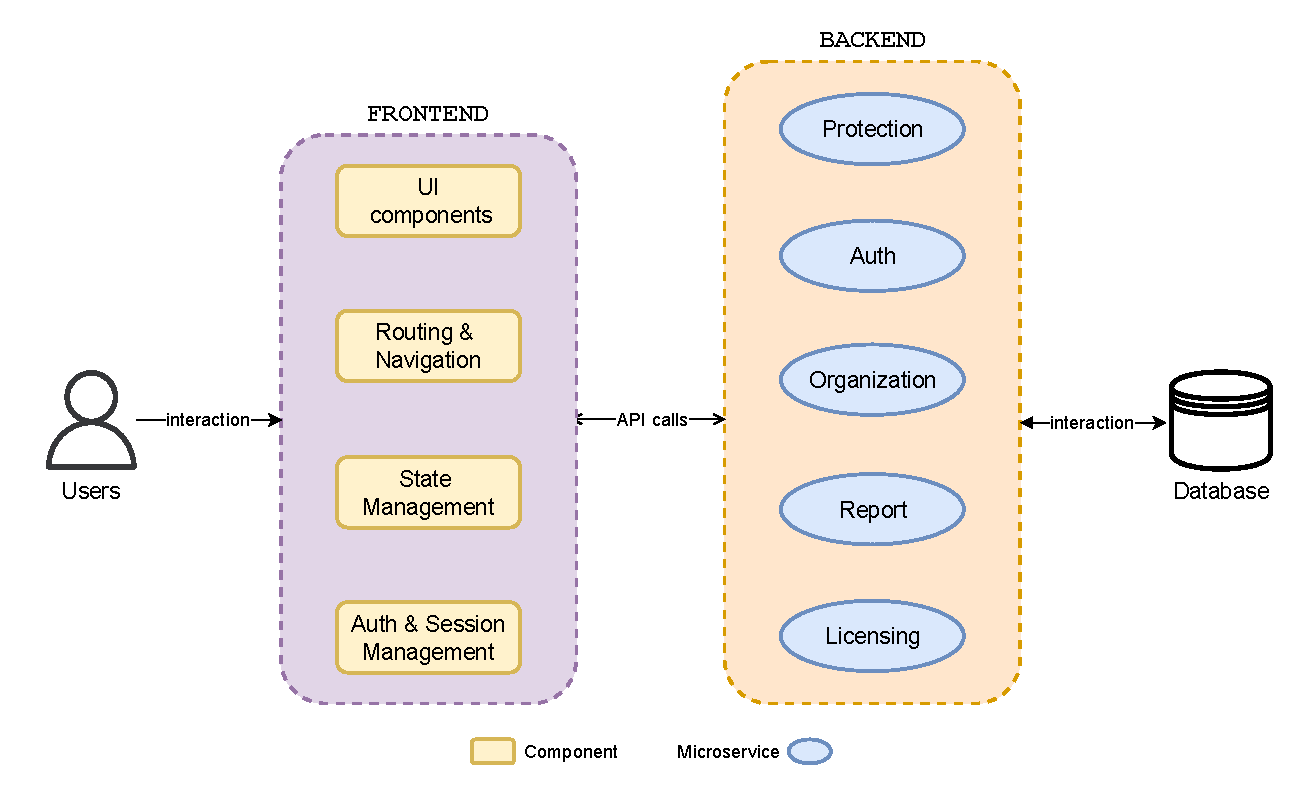
\includegraphics[width=1\textwidth]{figures/system-architecture.pdf}
  \caption{Architettura generale del sistema.}
  \label{fig:system-architecture}
\end{figure}

\subsection{Frontend}
Il frontend è stato progettato come una Single-Page Application\footnote{\url{https://link.springer.com/chapter/10.1007/978-1-4302-6674-7_1}} (SPA), scelta che consente di offrire agli utenti un'esperienza fluida ed un accesso rapido da qualsiasi browser, senza bisogno di installare nessun applicativo. Questo microservizio si occupa esclusivamente della logica di presentazione, implementando l'interfaccia grafica e gestendo l'interazione con gli utenti finali. Infatti, tutte le operazioni di elaborazione dei dati, come le computazioni o la gestione delle regole di business, sono demandate al backend.

L'architettura del frontend segue un approccio modulare, in cui ogni pagina e componente è organizzato secondo una struttura gerarchica. Ciò consente di mantenere l'architettura chiara e scalabile, facilitando l'estensione del sistema e la gestione delle singole sezioni dell'applicazione.

Per garantire un design coerente e accelerare lo sviluppo dell'interfaccia, è stato adottato un template grafico altamente personalizzabile. Questo approccio ha consentito di ridurre i tempi di progettazione dell’interfaccia grafica, mantenendo al contempo la flessibilità necessaria per adattare l’aspetto grafico alle esigenze specifiche del progetto.

\subsection{Backend}
Come già accennato, il backend non è stato concepito come un unico servizio monolitico, ma si è optato per una suddivisione in più microservizi, ciascuno responsabile di una specifica funzionalità o modulo del sistema. La definizione di questi microservizi è stata guidata dall'analisi del dominio (\Cref{sec:domain-analysis}), individuando le principali entità e le loro responsabilità all'interno dell'architettura complessiva. Questo approccio ha permesso di modellare il backend in modo coerente con le esigenze del sistema, garantendo una chiara separazione delle responsabilità e facilitando l'evoluzione futura della piattaforma.

Di seguito, vengono descritti i principali microservizi di cui il backend è composto:
\paragraph{Auth}
Il microservizio \texttt{auth} è responsabile dell'autenticazione e dell'autorizzazione degli utenti. L'autenticazione è implementata attraverso un meccanismo basato su token, che consente di gestire sessioni sicure senza la necessità di mantenere uno stato lato server.
L'autorizzazione, invece, fornisce un sistema per determinare se un utente ha i permessi necessari per eseguire una determinata azione. Questa valutazione si basa sul ruolo dell'utente e sulla licenza a lui associata, garantendo così un controllo granulare sugli accessi alle funzionalità della piattaforma.

\paragraph{Report}
Il microservizio \texttt{report} gestisce la generazione e la visualizzazione dei report relativi alle attività di filtraggio DNS. Nella prima versione del sistema, questa funzionalità è limitata alla visualizzazione di report specifici per gli MSP. Questo microservizio si interfaccia con il database per raccogliere e aggregare i dati necessari, fornendo agli utenti una panoramica dettagliata sull'attività di filtraggio e sull'efficacia delle policy applicate.

\paragraph{Organization}
Il microservizio \texttt{organization} è un componente chiave per l'implementazione della multiutenza. Esso si occupa di gestire tutte le operazioni CRUD sugli utenti, consentendo di creare nuovi account, modificare i ruoli, nonché rimuovere utenti dalle organizzazioni.
Grazie a questo servizio, più utenti possono essere associati a un'unica organizzazione con livelli di accesso differenziati, migliorando la flessibilità e la gestione delle autorizzazioni.

\paragraph{Protection}
Il microservizio \texttt{protection} è responsabile della gestione delle policy di protezione applicate agli utenti e alle organizzazioni. Questo servizio permette di creare, modificare ed eliminare i profili di protezione, ossia insiemi di regole che determinano quali contenuti possono essere filtrati o consentiti.
Inoltre, gestisce la creazione e l’amministrazione dei profili condivisi, che consentono di applicare una configurazione comune a più clienti senza dover definire manualmente le stesse regole per ciascuno di essi.

\paragraph{Licensing}
Il microservizio \texttt{licensing} si occupa della gestione delle licenze associate agli utenti e alle organizzazioni. Attraverso questo servizio, è possibile visualizzare lo stato delle licenze attive, gestire le assegnazioni e monitorare la loro scadenza.
Questo microservizio è essenziale per garantire che ogni utente abbia accesso solo alle funzionalità previste dal proprio piano, permettendo un controllo efficace sui livelli di servizio offerti.

\subsubsection{Architettura a livelli}
I microservizi appena discussi adottano un'architettura uniforme, basata sull'esposizione di API REST, garantendo una progettazione modulare e scalabile. Tale struttura consente di mantenere indipendenti le diverse componenti del sistema, facilitando la manutenzione e l'evoluzione del software. Ogni microservizio è organizzato in più livelli, ciascuno con responsabilità ben definite, come illustrato in \Cref{fig:microservice-architecture}:

\begin{itemize}
  \item \textbf{Routes}: rappresenta il punto di ingresso delle richieste HTTP. Questo livello si occupa di applicare eventuali middleware, come quello per la gestione dell'autenticazione, e di indirizzare le richieste verso il controller appropriato, in base al metodo HTTP e al percorso richiesto.

  \item \textbf{Controllers}: ricevono le richieste dai Routes, validano i parametri in ingresso e delegano l'elaborazione ai servizi applicativi. Una volta ottenuto il risultato, i controller generano la risposta HTTP da restituire al client.

  \item \textbf{Services}: costituiscono il livello di business logic, elaborando i dati e orchestrando le operazioni necessarie. Questo livello intermedio permette di mantenere separata la logica di dominio dall'accesso ai dati, garantendo maggiore modularità e riusabilità del codice.

  \item \textbf{Repositories}: forniscono un'interfaccia per l'accesso ai dati, eseguendo operazioni di lettura e scrittura sul database. Questo livello è responsabile esclusivamente della gestione dei dati.

  \item Database: sebbene non sia parte integrante dell'architettura dei microservizi, rappresenta il livello di persistenza su cui vengono eseguite le operazioni di lettura e scrittura da parte dei Repository.
\end{itemize}

\begin{figure}
  \centering
  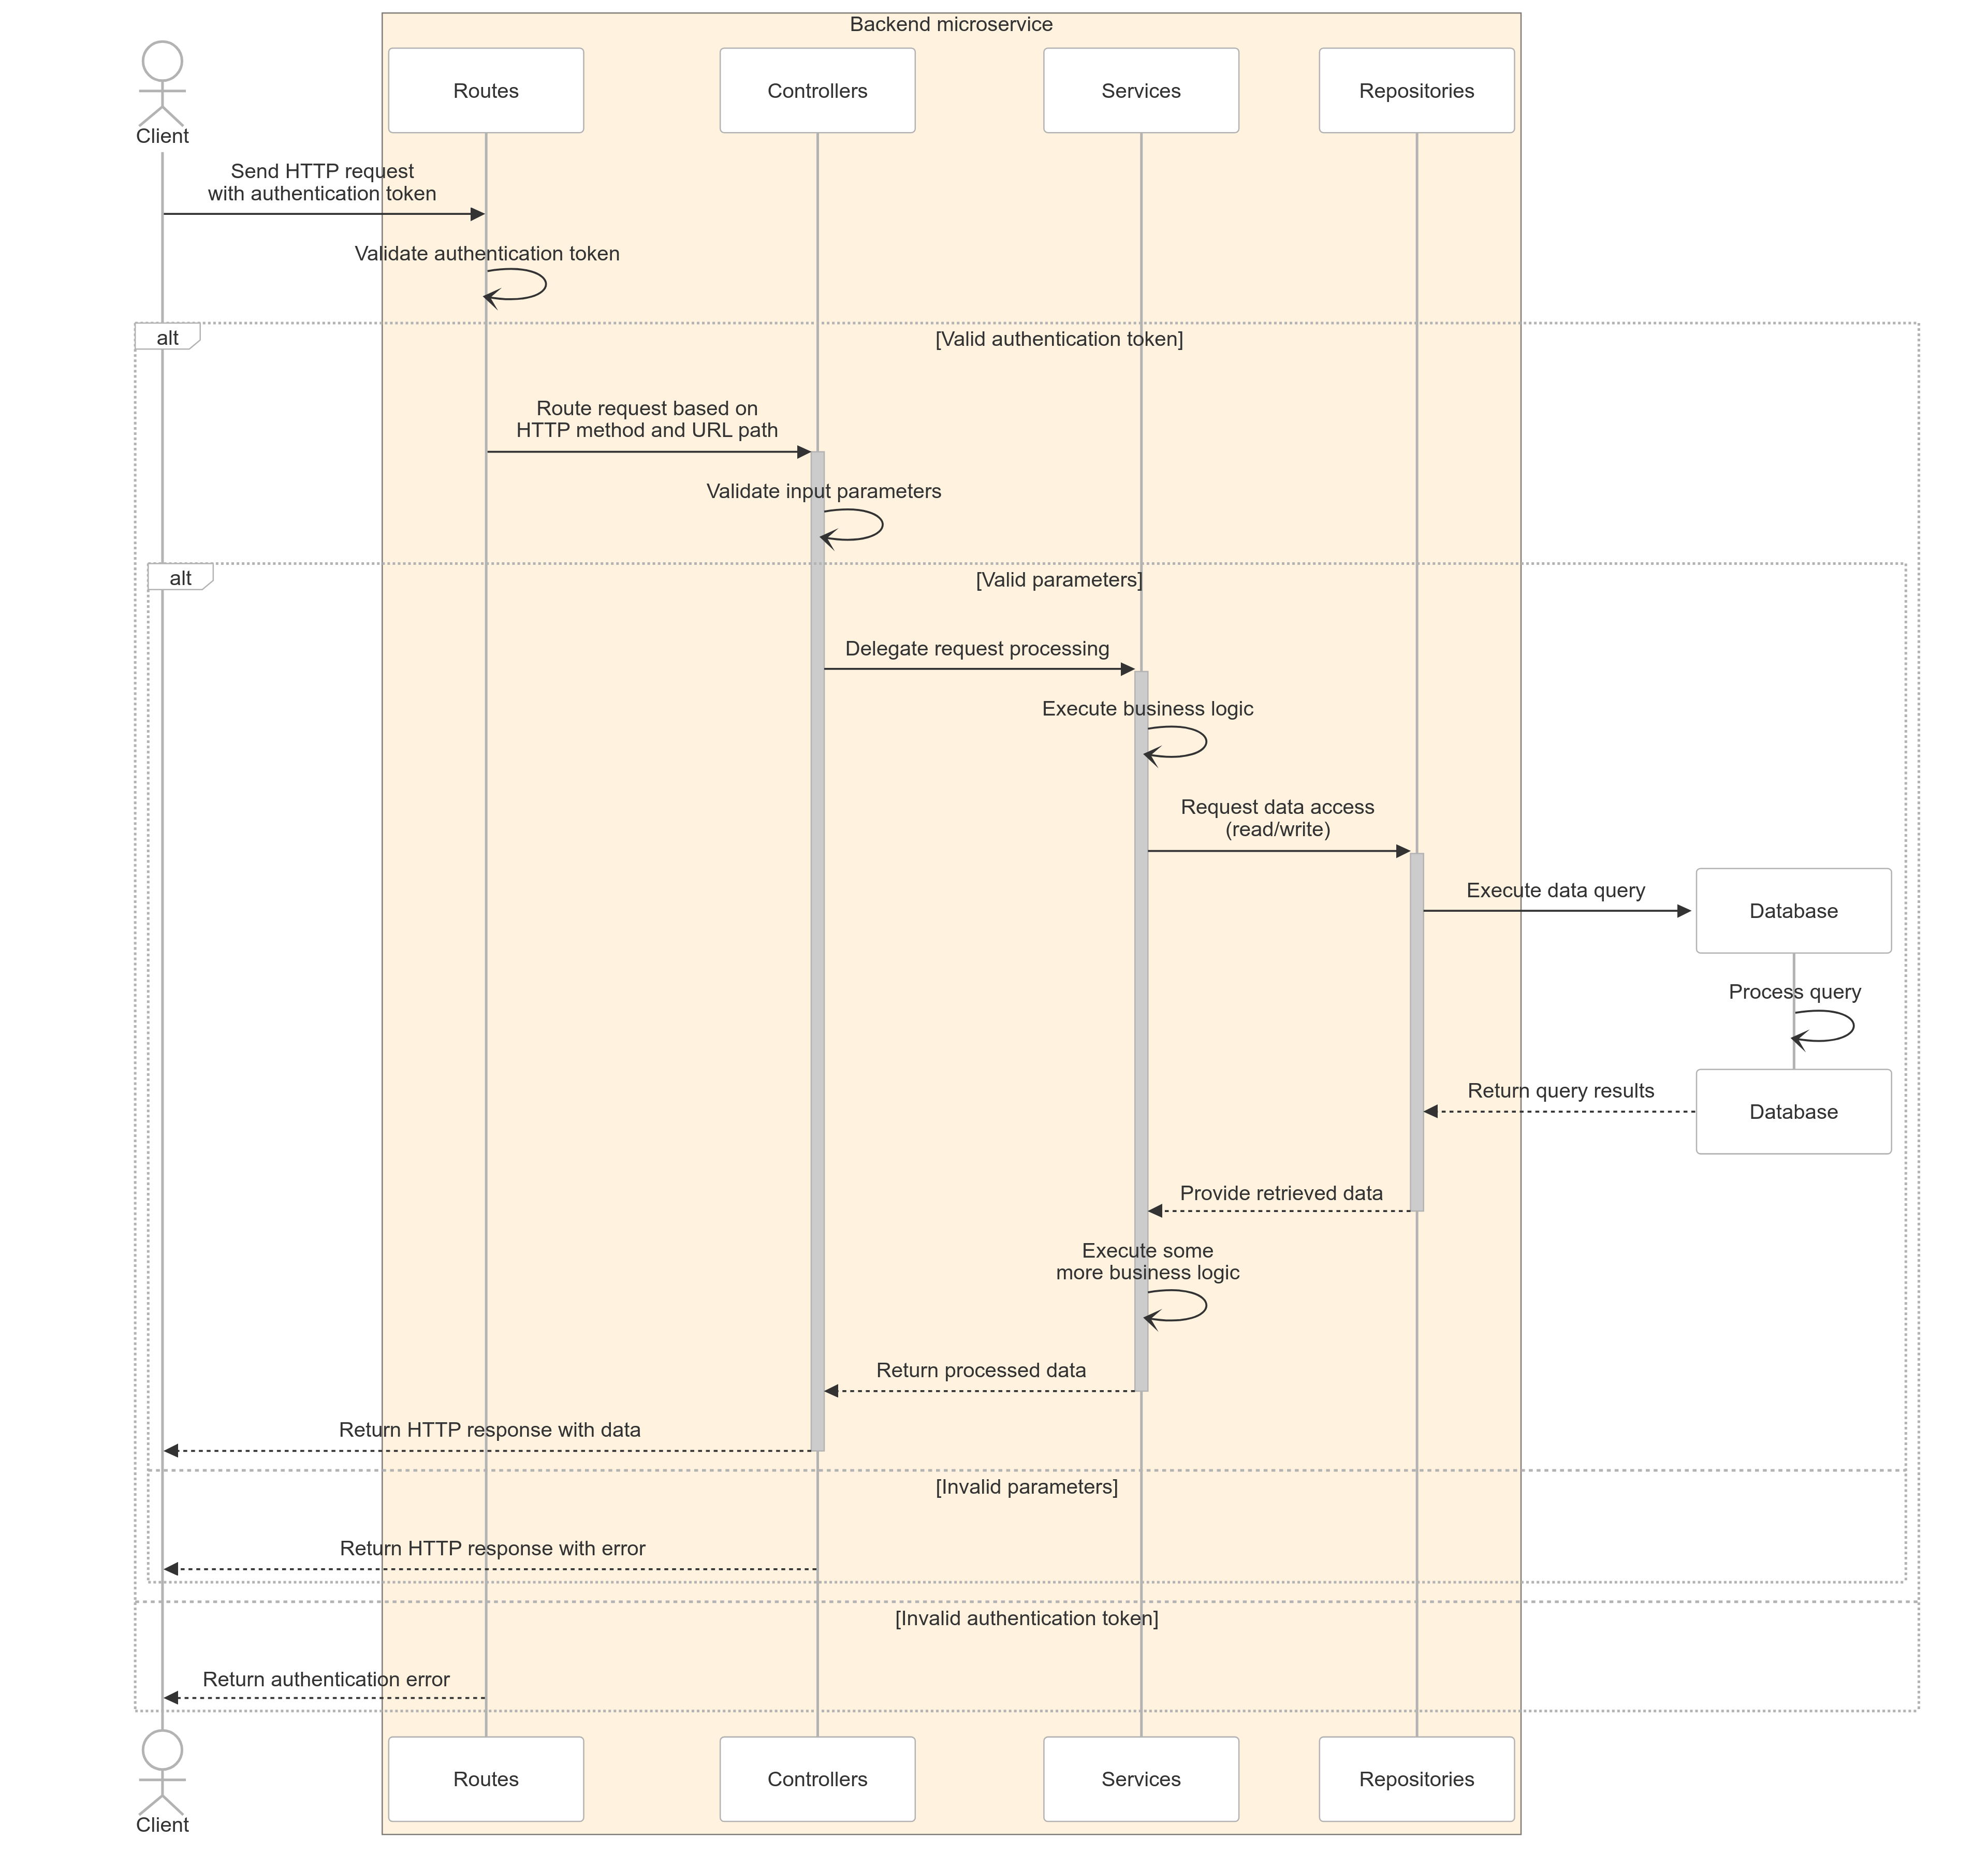
\includegraphics[width=1\textwidth]{figures/microservice-architecture.png}
  \caption{Diagramma di sequenza UML relativo all'architettura a livelli dei microservizi del backend.}
  \label{fig:microservice-architecture}
\end{figure}

Questa suddivisione in livelli garantisce una chiara separazione delle responsabilità, migliorando la manutenibilità e la scalabilità del sistema. Inoltre, consente di evolvere il backend in modo strutturato, rendendo più semplice l'aggiunta di nuove funzionalità o modifiche alle logiche applicative senza impattare gli altri componenti.

\subsection{Scelte tecnologiche}
Le tecnologie utilizzate per l'implementazione del nuovo sistema erano già state definite prima dell'inizio del presente contributo di tesi. Tuttavia, la loro adozione può essere motivata sulla base di considerazioni tecniche e di opportunità.

Per l'intero sistema, sia frontend che backend, è stato scelto il linguaggio TypeScript\footnote{\url{https://www.typescriptlang.org}}, che combina la flessibilità e la vasta disponibilità di librerie di JavaScript con i vantaggi di un linguaggio tipizzato. Grazie a TypeScript, è stato possibile sviluppare entità e funzionalità più robuste rispetto a un'implementazione in JavaScript puro, riducendo il rischio di errori a runtime. Il sistema di tipizzazione consente di individuare molteplici errori già in fase di compilazione, generando file JavaScript più affidabili e sicuri.

Come sistema di gestione delle dipendenze, si è optato per \texttt{pnpm}\footnote{\url{https://pnpm.io}}, un package manager che offre un'alternativa più efficiente rispetto al classico \texttt{npm} e \texttt{yarn}. Questo strumento si distingue per la sua capacità di ottimizzare l'uso dello spazio su disco condividendo le dipendenze tra i progetti, evitando duplicazioni inutili e riducendo significativamente i tempi di installazione. Inoltre, garantisce una gestione più affidabile delle dipendenze grazie al meccanismo di \textbf{store globale}, che assicura un'integrità maggiore rispetto agli altri gestori. La scelta di \texttt{pnpm} è stata adottata in maniera uniforme per garantire coerenza tra frontend e backend, migliorando l'efficienza del processo di sviluppo.

\subsubsection{Tecnologie del frontend}
Il frontend è stato sviluppato utilizzando Next.js\footnote{\url{https://nextjs.org}}, un framework basato su React. La scelta di React\footnote{\url{https://react.dev}} è stata dettata dalla volontà di mantenere la filosofia del sistema legacy, che forniva il pannello sotto forma di web application, e dalla sua combinazione tra ampia diffusione, efficienza e curva di apprendimento bilanciata. Tuttavia, piuttosto che utilizzare React in modo standalone, si è preferito adottare un framework che ne ottimizzasse l’utilizzo. Next.js è stato selezionato per le sue funzionalità avanzate, tra cui il pieno supporto a TypeScript e la gestione automatizzata di operazioni come il bundling e la compilazione, consentendo agli sviluppatori di concentrarsi sulla logica applicativa senza preoccuparsi della configurazione dell'ambiente di sviluppo.

Come strategia di routing delle pagine, si è scelto di utilizzare App Router\footnote{\url{https://nextjs.org/docs/app}}, il sistema di routing integrato in Next.js. Questo approccio permette di definire le rotte dell'applicazione in modo strutturato, organizzando il codice in base alla gerarchia delle directory. Inoltre, offre supporto per il rendering lato server, migliorando la flessibilità nella gestione e nel caricamento dei componenti.

Dal punto di vista grafico, la scelta del template TailAdmin\footnote{\url{https://tailadmin.com}} come base di partenza è stata motivata dalla sua somiglianza con il design desiderato per il nuovo sistema. La disponibilità di schermate predefinite e componenti riutilizzabili ha accelerato lo sviluppo dell’interfaccia, mentre la sua natura open source ha garantito massima flessibilità, permettendo modifiche e personalizzazioni senza vincoli.

\subsection{Tecnologie del backend}
Tutti i microservizi del backend utilizzano il framework web Express\footnote{\url{https://expressjs.com}} per esporre le loro API REST. Questa scelta è stata dettata dalla leggerezza e rapidità di tale libreria, oltre alla sua capacità di gestire le rotte in modo intuitivo e modulare. Express consente di definire una gerarchia di routing chiara, facilitando la suddivisione delle responsabilità tra i vari livelli dell'architettura. Inoltre, supporta l'integrazione di middleware personalizzati, aumentando la flessibilità nella gestione delle logiche applicative, come l'autenticazione e la validazione delle richieste.

Per i meccanismi di autenticazione, si è optato per un sistema basato su JSON Web Token\footnote{\url{https://datatracker.ietf.org/doc/html/rfc7519}} (JWT). Questa soluzione è ampiamente diffusa grazie alla sua semplicità di implementazione e alla possibilità di essere utilizzata in ambienti scalabili e distribuiti senza la necessità di mantenere uno stato centralizzato per le sessioni utente. A condizione che venga implementata correttamente, JWT garantisce un elevato livello di sicurezza, permettendo un controllo efficiente sugli accessi e l'integrazione con i microservizi in maniera indipendente.

Per quanto riguarda la gestione dell’accesso ai dati, si è scelto di adottare un ORM (Object-Relational Mapping) per semplificare l’interazione tra il backend e il database, evitando la necessità di scrivere manualmente query SQL complesse all’interno del codice applicativo. In particolare, la scelta è ricaduta su Prisma\footnote{\url{https://www.prisma.io}}, che si differenzia dagli Object-Relational Mapping tradizionali per il suo approccio dichiarativo. Più in dettaglio, a differenza degli ORM convenzionali, che mappano le tabelle del database su classi del linguaggio di programmazione, Prisma utilizza uno schema dichiarativo chiamato \textit{Prisma Schema} come unica fonte di verità per la struttura del database e dei modelli dell’applicazione. Questo consente una gestione più chiara e coerente dei dati, evitando le problematiche legate all'incompatibilità tra il modello a oggetti e quello relazionale.

Dal punto di vista della programmazione, Prisma fornisce una libreria lato client che permette di eseguire operazioni di lettura e scrittura sul database in modo tipizzato e sicuro, senza la necessità di gestire manualmente istanze di modelli complessi.

\subsubsection{Scelte tecnologiche del database}
Il nuovo sistema adotta un database relazionale con tecnologia PostgreSQL, scelta dettata principalmente dalla necessità di garantire la compatibilità con i dati gestiti dal sistema legacy, che utilizza lo stesso DBMS. Oltre a questo requisito, PostgreSQL è stato selezionato per le sue caratteristiche di affidabilità, scalabilità e performance, rendendolo una soluzione solida per applicazioni che devono gestire un elevato volume di dati e richieste concorrenti.

\section{Funzionalità chiave}
\subsection{Multiutenza e gestione degli utenti}
Nel nuovo sistema, la multiutenza si riferisce alla possibilità per un'organizzazione di disporre di molteplici credenziali di accesso, consentendo a diversi utenti di accedere al pannello di configurazione del filtro. Essi, hanno quindi la possibilità di amministrarne le caratteristiche o monitorare le statistiche, in base al loro ruolo. Questo rappresenta un notevole miglioramento rispetto al sistema precedente, in cui ogni cliente disponeva di un singolo account con permessi di amministratore. Tale limitazione risultava problematica in particolar modo per le organizzazioni più strutturate, che necessitavano di un accesso distribuito tra più figure con differenti livelli di autorizzazione.

\subsubsection{Modello attuale di gestione degli utenti}
Attualmente, come già spiegato nella \Cref{sec:domain-analysis}, gli utenti esistono solo nel contesto dell'organizzazione di cui fanno parte. Ogni organizzazione, infatti, al momento della creazione, dispone di un account utente con ruolo di amministratore (Admin). Quest'ultimo ha la possibilità di creare altri utenti, assegnando loro un ruolo specifico e un'organizzazione di appartenenza. Tale organizzazione può essere la stessa di chi effettua la creazione, oppure una delle organizzazioni gestite (nel caso di utenti appartenenti a MSP o Dealer). Inoltre, l'Admin può modificare le informazioni di qualsiasi utente della propria gerarchia, nonché eliminarlo.

\subsubsection{Gestione dell'autenticazione e della sessione}
L'autenticazione nel backend segue il meccanismo JWT, garantendo sicurezza e scalabilità nella gestione degli accessi. Le password degli utenti, prima di essere memorizzate nel database, vengono sottoposte a \textit{hashing} mediante la funzione \texttt{bcrypt}\footnote{\url{https://www.usenix.org/legacy/events/usenix99/provos/provos_html/index.html}}, utilizzando un ``fattore di lavoro'' pari a 10, che determina il numero di iterazioni dell'algoritmo e influisce sul tempo necessario per generare l'output. Questo parametro rende più oneroso il calcolo dell'\textit{hash}, ed il valore scelto aumenta la resistenza agli attacchi di forza bruta senza compromettere le prestazioni del sistema.

Durante il login, il backend genera e restituisce due token, in accordo con JWT: l'\textit{access token}, incluso nel corpo della risposta, e il \textit{refresh token}, inviato come cookie HTTP-only. Il primo incorpora le informazioni essenziali per l'identificazione dell'utente, tra cui il suo ID, l'email e il ruolo, permettendo al backend di verificare le autorizzazioni senza dover interrogare il database a ogni richiesta. Il secondo, invece, consente di ottenere un nuovo \textit{access token} senza costringere l'utente a eseguire nuovamente l'autenticazione, migliorando così l'esperienza d'uso.

Questa strategia non solo incrementa la sicurezza, evitando l’esposizione dei \textit{refresh token} nel codice lato client, ma semplifica anche la gestione per il frontend. Infatti, grazie all'uso dei cookie HTTP-only, il browser si occupa automaticamente dell'invio del \textit{refresh token} nelle richieste al backend, riducendo il rischio di furti di credenziali e migliorando la protezione complessiva del sistema.

\subsubsection{Limitazioni e aspetti da migliorare}
Per garantire una corretta gestione dell'autorizzazione, si è deciso di adottare un modello basato su Role-Based Access Control\footnote{\url{https://www.sciencedirect.com/science/article/abs/pii/S0167404803006096}} (RBAC). Tuttavia, tale sistema non è ancora stato implementato nella sua completezza.

Attualmente, sono previste solo due tipologie di utenti, Admin e ReadOnly, ma senza una distinzione effettiva nei permessi tra le due categorie. Gli utenti ReadOnly, infatti, possono eseguire le stesse operazioni degli Admin. Questa configurazione rappresenta una soluzione provvisoria, in attesa dell'introduzione di un sistema RBAC più strutturato. Una volta implementato, gli utenti ReadOnly saranno limitati esclusivamente alla visualizzazione di report e statistiche, senza la possibilità di apportare modifiche.

Oltre alla gestione dei ruoli, un ulteriore livello di complessità deriva dal fatto che i permessi non dipendono esclusivamente dal ruolo assegnato all'utente, ma anche dai privilegi associati all’organizzazione di appartenenza, i quali a loro volta sono influenzati dalla tipologia di licenza in uso. Per affrontare questa complessità, è prevista l'implementazione di un sistema basato su una lista di permessi derivanti da questi fattori. Tali permessi verranno poi aggregati e consolidati dal backend durante il processo di autorizzazione, restituendo al client solo il fatto che l'utente abbia o meno il permesso di eseguire una determinata azione.

Questo sistema di permessi sarà applicato sia nel frontend, per regolare l'accesso alle pagine e ai componenti dell'interfaccia utente, sia nel backend, per proteggere le API e le operazioni disponibili per ciascun utente. In questo modo, sarà possibile garantire un accesso controllato e coerente su tutti i livelli del sistema, migliorando la sicurezza e l’affidabilità del processo di autorizzazione.

\subsection{Gestione degli errori}
Uno degli aspetti chiave della progettazione del nuovo sistema riguarda la definizione di un meccanismo di gestione degli errori strutturato e centralizzato. Questo sistema, sviluppato appositamente nell’ambito del tirocinio che ha portato alla presente tesi, consente di rappresentare e trattare in modo coerente le diverse tipologie di errore, garantendo uniformità tra backend e frontend e migliorando l’esperienza utente.

L'obiettivo principale di questa soluzione è evitare una gestione dispersiva e poco strutturata degli errori, introducendo un modello tipizzato e scalabile. Il sistema consente di differenziare gli errori in base al contesto e alla loro natura, assicurando che ogni anomalia sia rappresentata con un formato chiaro e prevedibile. Questo approccio consente inoltre di evitare l'esposizione di informazioni sensibili e di mantenere la logica di gestione degli errori separata dalle altre componenti del sistema.

\subsubsection{Gestione degli errori nel backend}
Il sistema di gestione degli errori nel backend è stato progettato attorno a una gerarchia di classi che permette di categorizzare le diverse tipologie di errore. Alla base vi è una classe astratta che definisce una struttura comune, fornendo un codice identificativo, un codice di stato HTTP e un eventuale insieme di dettagli aggiuntivi. Le classi derivate rappresentano errori specifici dell’applicazione e sono strutturate per coprire due aspetti principali: da un lato, scenari generici come accesso non autorizzato o errori interni del server; dall’altro, errori strettamente legati alle entità del dominio applicativo. In quest’ultimo caso, ogni entità è associata a una serie di errori tipici, come \texttt{UserNotFound} per indicare l’assenza di un utente richiesto o \texttt{UserCreateError} per segnalare un problema nella creazione di un nuovo utente.

Per mantenere un formato coerente, tutti gli errori seguono una mappatura predefinita, che associa ogni codice identificativo a un insieme strutturato di dettagli. Questa soluzione garantisce che ogni errore disponga delle informazioni necessarie per essere compreso dal frontend senza ambiguità. La gestione delle eccezioni è completata da un middleware centralizzato, che intercetta gli errori a tutti i livelli del backend e restituisce una risposta strutturata, includendo solo le informazioni rilevanti per il client.

Grazie a questa architettura, la gestione degli errori nel backend risulta modulare ed estensibile, permettendo di aggiungere nuove tipologie di errore senza impattare il resto del sistema.

\subsubsection{Gestione degli errori nel frontend}
Il sistema di gestione degli errori è stato progettato in modo da garantire una perfetta integrazione con il frontend. In particolare, il codice d'errore e i dettagli aggiuntivi forniti dal backend consentono al frontend di costruire messaggi chiari e contestualizzati per l'utente, senza che le stringhe siano \textit{hard-coded} nel backend.

Un aspetto rilevante della progettazione è la compatibilità con il sistema di multilingua del frontend. La struttura dei codici di errore, infatti, segue la stessa organizzazione delle directory utilizzate per la localizzazione delle stringhe, rendendo immediata la traduzione del messaggio in base alla lingua selezionata dall'utente. Questo permette di generare notifiche e avvisi coerenti senza necessità di duplicare la logica di gestione degli errori in più parti del sistema.

\section{Miglioramento del database}
Il database del nuovo sistema è stato quasi completamente rinnovato come parte integrante del processo di reingegnerizzazione in corso. Questo intervento è stato reso possibile dal cambio di strategia descritto nella \Cref{sec:transizione}, che ha eliminato la necessità di una coesistenza tra il vecchio e il nuovo sistema, optando invece per una transizione netta.

L’assenza di vincoli legati alla retrocompatibilità ha permesso di riprogettare la base dati in accordo con l’analisi del dominio, affrontando e risolvendo le criticità presenti nella precedente modellazione. Questa libertà ha consentito di introdurre una struttura più coerente e scalabile, ottimizzando la gestione delle informazioni e predisponendo il sistema per l’integrazione di nuove funzionalità.

\subsection{Struttura della base dati}
La seguente analisi descrive l'architettura del nuovo database, mettendo in evidenza le principali differenze rispetto al sistema legacy. Le entità saranno presentate in gruppi tematici, organizzati in base alla loro funzione, fornendo una visione strutturata delle relazioni e delle caratteristiche di ciascuna componente del modello dati. In \Cref{fig:database-schema} è riportato lo schema concettuale del database, che rappresenta la struttura delle entità e delle relazioni principali.

\begin{sidewaysfigure}
  \centering
  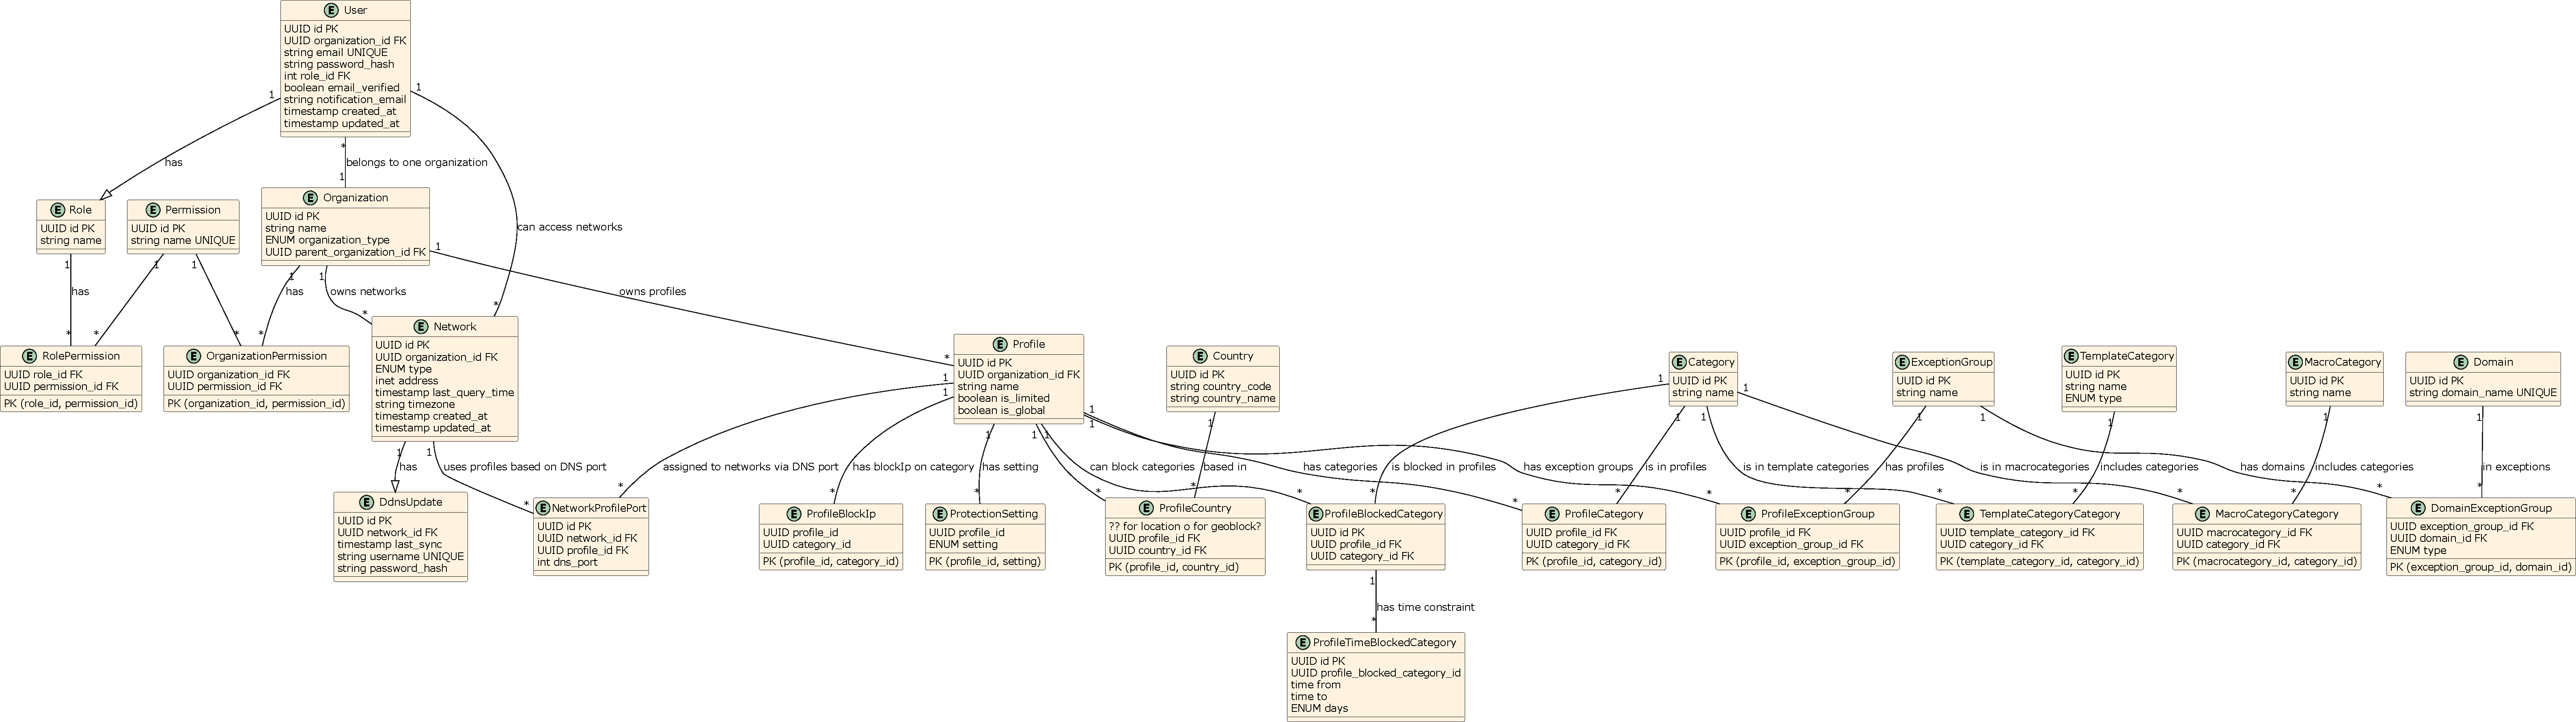
\includegraphics[width=1\textwidth]{figures/new_database_schema.pdf}
  \caption{Diagramma ER relativo al database del nuovo sistema.}
  \label{fig:database-schema}
\end{sidewaysfigure}

\subsubsection{Gestione delle organizzazioni, degli utenti e dei permessi}
La gestione delle organizzazioni e degli utenti è centrale nel modello del database, in quanto permette di strutturare il sistema in modo scalabile e multi-tenant. Ogni organizzazione definisce un'unità amministrativa indipendente, all'interno della quale operano utenti con ruoli e permessi specifici.

\paragraph{Struttura gerarchica delle organizzazioni}
Il database prevede la possibilità di modellare relazioni gerarchiche tra organizzazioni, consentendo la gestione di scenari in cui un'entità superiore controlla più sotto-organizzazioni. Questo è realizzato attraverso una relazione auto-referenziale sull'entità Organization. Pertanto, ogni organizzazione può opzionalmente riferirsi a un'organizzazione genitore, creando così una struttura ad albero. Tale approccio è particolarmente utile nei casi in cui un provider di servizi (Dealer o MSP) debba gestire clienti separati, mantenendo al contempo un controllo centralizzato.

\paragraph{Associazione tra utenti e organizzazioni}
Gli utenti nel sistema appartengono a una specifica organizzazione, stabilendo un legame chiaro tra le entità amministrative e gli individui che vi operano. Questo vincolo è fondamentale per garantire che ogni utente possa accedere solo ai dati e alle configurazioni pertinenti alla propria organizzazione, rispettando i livelli di isolamento tra clienti diversi.

Un aspetto critico del modello è la gestione dei ruoli e dei permessi, che determinano le operazioni che un utente può eseguire all’interno della propria organizzazione o di quelle subordinate. Il ruolo di ciascun utente viene interpretato direttamente dal backend del sistema e regola le azioni disponibili nell’applicazione, garantendo un controllo granulare sull’accesso alle funzionalità.

\paragraph{Gestione dei permessi}
Nel database vengono gestite due tipologie di permessi, che operano su livelli differenti:
\begin{itemize}
  \item \textbf{Permessi di ruolo}: definiti staticamente all'interno del backend e assegnati in base alla tipologia dell’utente. Essi determinano le operazioni consentite all’interno del sistema, come la possibilità di apportare modifiche ai parametri del filtro o visualizzare determinate informazioni.
  \item \textbf{Permessi di organizzazione}: memorizzati nel database ma gestiti dalla \textit{customer area}, un sistema esterno a quello in esame. Questi permessi sono definiti sulla base della licenza associata all'organizzazione e regolano le funzionalità accessibili per gli utenti al suo interno. Sebbene non siano amministrati direttamente dal backend, risultano fondamentali per il servizio di autorizzazione, che li utilizza per stabilire se un utente ha il diritto di eseguire una determinata operazione.
\end{itemize}

\subsubsection{Gestione delle reti e dei profili di protezione}
Il modello di database adotta un approccio basato sui \emph{profili}, che rappresentano l’unico punto in cui vengono definite le policy di filtraggio. Le reti non contengono direttamente regole di protezione, ma si associano a uno o più profili per determinare quali configurazioni di sicurezza applicare.

\paragraph{Gestione delle reti}
Ogni organizzazione può registrare una o più reti, che rappresentano gli indirizzi IP dai quali provengono le richieste al sistema. Una delle principali innovazioni introdotte in questa modellazione è il supporto alla notazione CIDR, che permette di rappresentare un intero intervallo di indirizzi IP con una sola entry nel database. Questo migliora significativamente l’efficienza del sistema, riducendo il numero di righe necessarie rispetto al modello precedente, in cui ogni indirizzo IP veniva memorizzato singolarmente, anche se appartenente allo stesso range.

Per supportare scenari in cui gli indirizzi IP di una rete cambiano dinamicamente, è presente un meccanismo di aggiornamento tramite \emph{DDNS}. Il database memorizza le informazioni necessarie per gestire queste variazioni, includendo dati di autenticazione e timestamp relativi all’ultimo aggiornamento della rete registrata.

\paragraph{Profili di protezione}
Nel nuovo database, i profili di protezione sono modellati come entità indipendenti, associate a una specifica organizzazione, ma con la possibilità di essere condivise con le organizzazioni ad essa subordinate. Questo meccanismo è implementato tramite un attributo che indica se un profilo è ereditabile all'interno della gerarchia. In tal caso, esso risulta visibile e utilizzabile anche per le organizzazioni figlie, evitando la duplicazione delle configurazioni di filtraggio.

\paragraph{Filtri e categorie di protezione}
Ogni profilo può essere associato a una serie di filtri di protezione, che regolano il blocco di contenuti in base a diverse tipologie di criteri. Il sistema prevede una tabella specifica per ciascun tipo di filtro, tra cui:
\begin{itemize}
  \item Blocco per categoria, per contenuto o singolo servizio;
  \item Abilitazione forzata di SafeSearch per i motori di ricerca;
  \item Limitazioni per indirizzi IP e domini.
\end{itemize}
La struttura del database prevede che per ogni opzione bloccata sia presente una riga separata. Ad esempio, se un profilo vieta l’accesso a cinque categorie di contenuti, la tabella relativa al blocco per categorie conterrà cinque righe distinte, ognuna riferita al profilo e alla categoria corrispondente.

Il database consente inoltre di definire i \emph{profili ristretti} attraverso un attributo dedicato, che indica se un profilo opera in modalità restrittiva. In questa configurazione, tutte le protezioni risultano attive di default, mentre l’accesso è consentito esclusivamente ai domini autorizzati. Sebbene l’informazione sia memorizzata nel database, la logica che governa il comportamento di questi profili è demandata al livello applicativo, che interpreta tale configurazione e applica le restrizioni di conseguenza.

\paragraph{Associazione dei profili alle reti}
L’assegnazione di un profilo a una rete avviene attraverso la coppia di server DNS utilizzata per le richieste. Questo meccanismo consente di determinare quale profilo debba essere applicato in base alla configurazione DNS impostata dall’amministratore, evitando così la necessità di separare fisicamente i dispositivi su reti diverse per applicare configurazioni differenti. Nel database, questo concetto è rappresentato dal termine \emph{porta}, una scelta terminologica che potrebbe apparire incoerente rispetto al suo significato tradizionale. Tuttavia, essa deriva da una versione precedente del sistema, in cui la selezione del profilo veniva effettivamente implementata sfruttando il numero di porta.

Questa modellazione permette quindi di gestire scenari avanzati in cui più profili possono coesistere sulla stessa rete, garantendo un elevato livello di flessibilità nella definizione delle policy di filtraggio e riducendo la necessità di configurazioni ridondanti.

\subsubsection{Gestione delle categorie e delle eccezioni}
Il nuovo database introduce una modellazione più strutturata delle categorie di contenuti e delle eccezioni, con l'obiettivo di migliorare la gestione delle configurazioni di filtraggio. Rispetto alla versione precedente, questa modellazione consente una maggiore flessibilità nella definizione delle policy, facilitando sia la gestione delle categorie predefinite sia la creazione di gruppi di eccezioni personalizzati.

\paragraph{Categorie e macrocategorie}
Le categorie rappresentano insiemi di domini classificati in base alla tipologia di contenuti, come \emph{social media}, \emph{streaming}, \emph{contenuti per adulti} e così via. Per migliorare la chiarezza e la gestione delle policy, ogni categoria appartiene a una \emph{macrocategoria}, che raggruppa più categorie affini.

L'introduzione delle macrocategorie non ha solo un valore organizzativo, ma viene sfruttata dal livello applicativo per semplificare le operazioni di configurazione. Grazie a questa struttura, un amministratore può decidere di abilitare o bloccare tutte le categorie appartenenti a una macrocategoria con un'unica azione, senza dover selezionare manualmente ogni singola voce.

\paragraph{Gestione delle categorie nei template}
Il database prevede anche la possibilità di definire insiemi preconfigurati di categorie attraverso il concetto di \emph{Template Category}. Un template di categoria rappresenta una configurazione standardizzata che include molteplici categorie, utile per velocizzare l’applicazione di policy predefinite.
%
L’utilizzo dei template permette di semplificare la gestione delle policy di filtraggio, evitando la necessità di selezionare manualmente ogni singola categoria. Un esempio pratico è la definizione di livelli di protezione preimpostati, con restrizioni progressive, che possono essere selezionati rapidamente senza dover configurare manualmente le singole categorie di contenuti. Questo approccio risulta particolarmente utile per fornire agli utenti meno esperti una modalità intuitiva per applicare politiche di filtraggio senza entrare nel dettaglio delle singole impostazioni.

\paragraph{Gestione avanzata delle eccezioni}
In questo contesto, una delle principali innovazioni rispetto al database precedente riguarda la gestione delle eccezioni. In passato, il sistema si basava esclusivamente su due liste distinte: una per i domini consentiti e una per i domini bloccati. Questo approccio era limitato, poiché ogni profilo doveva gestire separatamente le due liste, senza possibilità di organizzare le eccezioni in modo strutturato.

Il nuovo database introduce il concetto di \emph{gruppi di eccezioni}, che rappresentano insiemi di domini personalizzati contenenti sia elementi bloccati sia consentiti. Ogni gruppo può essere associato a uno o più profili, permettendo così di riutilizzare la stessa configurazione su più contesti senza dover ridefinire manualmente le liste di riferimento. La modellazione delle eccezioni si basa su tre entità principali:
\begin{itemize}
  \item \textbf{Gruppi di eccezioni}: rappresenta i gruppi di eccezioni, identificati da un nome.
  \item \textbf{Associazione tra profili e gruppi di eccezioni}: definisce la relazione tra i profili e i gruppi di eccezioni, consentendo di applicare la stessa configurazione a più profili.
  \item \textbf{Associazione tra domini e gruppi di eccezioni}: stabilisce l'associazione tra i domini e i gruppi di eccezioni, permettendo di definire quali appartengono a un gruppo specifico e se sono bloccati o consentiti.
  \item \textbf{Nomi di dominio}: rappresenta la lista dei domini inseriti tra le eccezioni.
\end{itemize}

Questa modellazione consente di gestire le eccezioni in modo molto più flessibile, permettendo di definire configurazioni granulari e riutilizzabili. Un’organizzazione può, ad esempio, creare un gruppo di eccezioni che include sia domini consentiti sia domini bloccati e applicarlo a più profili senza dover replicare manualmente le stesse configurazioni. Inoltre, grazie alla presenza dei profili condivisi, anche i gruppi di eccezioni associati a questi ultimi vengono ereditati dalle organizzazioni subordinate. Questo meccanismo consente di mantenere una gestione centralizzata delle eccezioni, assicurando coerenza tra le configurazioni applicate ai diversi livelli della gerarchia organizzativa.

\subsection{Linee guida per la migrazione dei dati}
Il processo di migrazione dei dati rappresenta un'operazione critica nel passaggio dal sistema legacy alla nuova infrastruttura, poiché coinvolge informazioni essenziali per il funzionamento del filtro DNS e per l'esperienza degli utenti. Affinché la transizione avvenga in modo efficace, il nuovo sistema dovrà essere già popolato con tutti i dati esistenti prima della sua messa in produzione, evitando così discontinuità operative o perdita di informazioni.

Attualmente, non è ancora stata definita nei dettagli la strategia di migrazione, poiché il nuovo sistema si trova in una fase iniziale di sviluppo. Tuttavia, è possibile delineare alcune considerazioni preliminari basate sul confronto tra la struttura del database legacy e la nuova modellazione dei dati. Queste riflessioni costituiscono un primo passo verso la progettazione di un processo di migrazione strutturato, che garantisca coerenza, integrità e compatibilità tra i due ambienti. Di seguito, verranno illustrate alcune linee guida fondamentali per la migrazione, organizzate in base alle principali entità del database. L'obiettivo è fornire un quadro chiaro delle trasformazioni necessarie e delle possibili strategie da adottare per assicurare una transizione fluida e priva di anomalie.

Prima di tutto, un aspetto fondamentale del processo in questione, che coinvolge ogni singola entità da trasferire, riguarda la gestione degli identificativi. Nel vecchio sistema, gli identificativi delle entità erano di tipo numerico e seguivano il tipo di dato \texttt{Decimal(1000, 1)}, di SQL. Nel nuovo sistema, si utilizzeranno invece identificativi di tipo \texttt{UUID} (Universally Unique IDentifier\footnote{\url{https://datatracker.ietf.org/doc/html/rfc9562}}), garantendo maggiore scalabilità e unicità. Di conseguenza, per ogni entità migrata, sarà necessario generare un nuovo UUID e aggiornare tutte le relazioni di conseguenza. Qualsiasi riferimento all'ID legacy dovrà essere tracciato temporaneamente in una tabella di mapping per facilitare il passaggio al nuovo schema.

\subsubsection{Migrazione delle organizzazioni e degli utenti}
La migrazione delle organizzazioni e degli utenti rappresenta un punto cruciale, in quanto bisogna passare da un sistema privo di multiutenza a uno in cui la funzionalità multi-tenant ha guidato lo sviluppo fin dall’inizio. Nel sistema legacy, non esisteva una distinzione tra organizzazione e utente: ogni riga della tabella \texttt{admin} con l'attributo \texttt{tipo = 1} rappresentava sia un cliente che il relativo utente amministratore. Questa struttura era possibile poiché vi era un singolo account per ogni cliente, eliminando la necessità di una separazione tra le due entità.

Nel nuovo sistema, invece, utenti e organizzazioni sono stati modellati come entità distinte. La migrazione dovrà quindi adattare i dati esistenti a questa nuova struttura, assicurando che ogni cliente del vecchio database venga convertito in una vera e propria organizzazione, con almeno un utente amministratore associato.

In particolare, il primo passo del processo di migrazione prevede la creazione delle organizzazioni nel nuovo sistema. Ogni riga della tabella \texttt{admin} con \texttt{tipo = 1} dovrà essere trasformata in una entry della tabella \texttt{organizations} del nuovo database. Gli attributi identificativi dell’organizzazione, come il nome, dovranno essere trasferiti e adattati alla nuova struttura.

Per ricreare la gerarchia delle organizzazioni, sarà necessario analizzare il valore del campo \texttt{cloud\_idfornitore} della tabella \texttt{admin}. Questo campo, se valorizzato, contiene l’indirizzo email dell’organizzazione padre, ovvero del cliente che gestisce l’entità in questione. Se il campo risulta vuoto, significa che l'organizzazione non è subordinata ad altre ed è quindi posizionata al livello più alto della gerarchia, come nel caso di dealer o MSP.
%
Nel nuovo sistema, l'associazione tra organizzazioni non avviene più tramite email, ma attraverso l'UUID dell'organizzazione padre. Pertanto, nel processo di migrazione, sarà necessario risolvere queste relazioni traducendo il valore di \texttt{cloud\_idfornitore} nel corrispondente UUID dell'organizzazione padre. Questo passaggio dovrà essere eseguito in due fasi:
\begin{enumerate}
  \item Creare tutte le organizzazioni migrando i dati dalla tabella \texttt{admin}, senza impostare subito il campo \texttt{parent\_organization\_id}.
  \item Dopo che tutte le organizzazioni sono state inserite nel nuovo database, aggiornare il campo \texttt{parent\_organization\_id} associando a ciascuna il corrispondente UUID dell'organizzazione padre, risolvendo la relazione tramite il valore presente in \texttt{cloud\_idfornitore}.
\end{enumerate}
Questa strategia garantisce che la gerarchia venga ricostruita correttamente senza incongruenze nella fase di migrazione.

Successivamente, per ogni organizzazione migrata, dovrà essere creato un utente amministratore corrispondente nella tabella \texttt{users}. L’utente dovrà essere associato all’organizzazione di riferimento tramite una chiave esterna, garantendo così una chiara relazione tra le due entità. Poiché nel sistema legacy l'utente e l'organizzazione coincidevano, sarà necessario separare logicamente i dati, assicurandosi che il nuovo sistema mantenga coerenza e integrità.

\subsubsection{Migrazione dei profili di configurazione}
La migrazione dei profili di configurazione rappresenta una delle operazioni più complesse, poiché il nuovo sistema ha introdotto il concetto di profili condivisi, modificando radicalmente la struttura e le modalità di associazione delle configurazioni di filtraggio.

Nel sistema legacy, i profili erano identificati tramite un codice profilo e associati ai clienti attraverso la tabella \texttt{admin}, con un legame statico e univoco. Questo significava che ogni profilo apparteneva esclusivamente a un singolo cliente, senza possibilità di essere condiviso tra più entità. Nel nuovo sistema, invece, i profili non sono più legati a una singola istanza del vecchio database, ma vengono associati direttamente alle organizzazioni, con la possibilità di essere riutilizzati dalle organizzazioni subordinate.

Sebbene sia teoricamente possibile effettuare un'analisi per identificare i potenziali profili da trasformare in condivisi, questa operazione risulta particolarmente complessa. Nel database legacy, infatti, non esiste un'informazione chiara e diretta che indichi se un profilo sia utilizzato da più clienti. Questo rende difficile stabilire automaticamente quali profili potrebbero essere condivisi senza introdurre ambiguità o errori nella migrazione.

Per garantire una transizione coerente, si può quindi procedere migrando tutti i profili esistenti e impostandoli inizialmente come non condivisibili, riproducendo fedelmente la configurazione che gli utenti avevano nel vecchio sistema. Una volta completata la migrazione, saranno gli stessi amministratori ad avere la possibilità di convertire i profili tradizionali in condivisi e riutilizzarli per più sottoclienti, sfruttando le nuove funzionalità del sistema.

\subsubsection{Migrazione delle categorie di blocco e delle eccezioni}
La migrazione delle categorie di blocco avverrà trasferendo i dati esistenti nelle nuove tabelle, assicurando che le associazioni tra profili e categorie rimangano invariate. Nel sistema legacy, l'associazione tra profilo e categorie era effettuata tramite il codice profilo collegato all'admin, mentre nel nuovo sistema viene utilizzato l'UUID del profilo. Di conseguenza, la migrazione dovrà prevedere la conversione dei riferimenti al codice profilo nel nuovo identificativo univoco, garantendo la coerenza con la nuova struttura dati.

Un aspetto più critico riguarda la gestione delle eccezioni, che nel nuovo sistema introduce gruppi riutilizzabili anziché liste statiche per ogni profilo. Per garantire una transizione coerente, la migrazione dovrà trasformare le eccezioni esistenti adattandole alla nuova struttura. Una possibile soluzione consiste nel creare un gruppo di eccezioni predefinito per ogni profilo, popolandolo con i domini bloccati e consentiti presenti nel vecchio database. Questo approccio mantiene le configurazioni originali, offrendo al contempo la maggiore flessibilità del nuovo sistema.

\subsubsection{Migrazione delle reti}
La migrazione delle reti richiede un processo di consolidamento degli indirizzi IP per adattarli alla nuova rappresentazione basata sulla notazione CIDR. Anziché memorizzare ogni singolo indirizzo come un’entry separata, il nuovo sistema consente di rappresentare un intero range di IP in modo compatto, riducendo la ridondanza e ottimizzando lo spazio di archiviazione.

Per garantire una transizione coerente, la migrazione dovrà prevedere la conversione degli indirizzi IP esistenti nella loro corrispondente rappresentazione CIDR. Questo comporta l’aggregazione degli indirizzi appartenenti allo stesso range e la loro trasformazione in un’unica entry nel nuovo database. Tale processo migliorerà le operazioni di gestione e ricerca delle reti, riducendo significativamente il numero di record memorizzati.
